\begin{figure}[H]
    \centering
    \begin{subfigure}{0.24\textwidth} 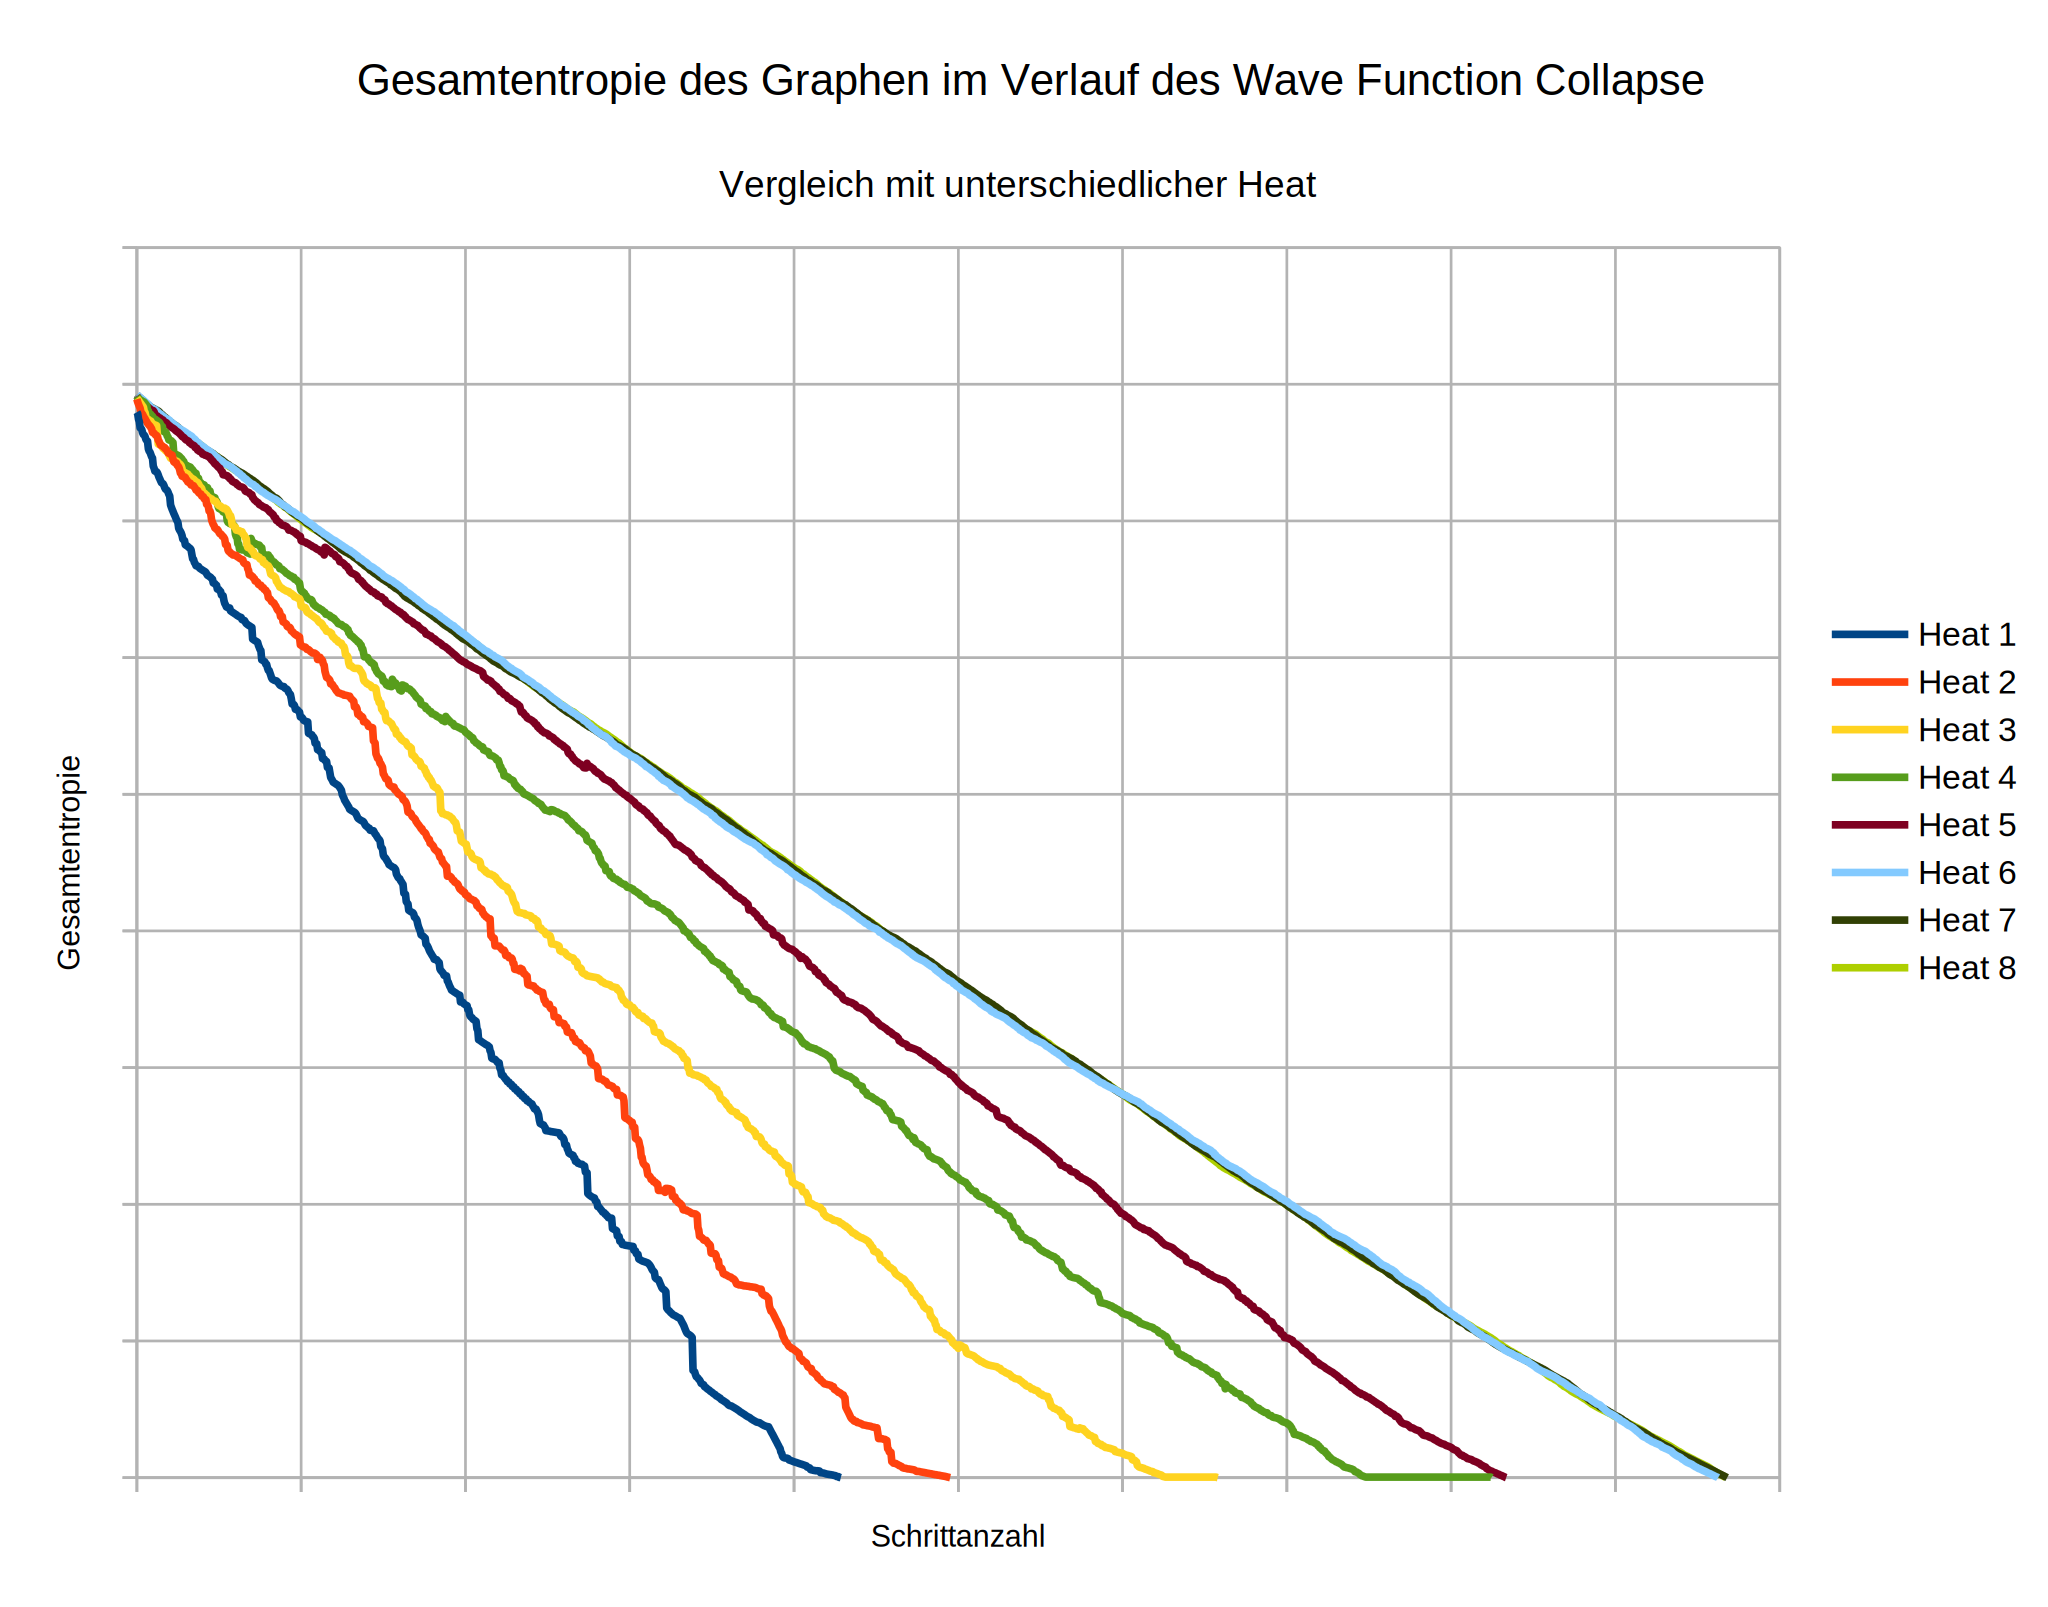
\includegraphics[width=\linewidth]{data/delaunay_voronoi/1.png}  \caption{} \end{subfigure}
    \begin{subfigure}{0.24\textwidth} \includegraphics[width=\linewidth]{data/delaunay_voronoi/2.png}  \caption{} \end{subfigure}
    \begin{subfigure}{0.24\textwidth} \includegraphics[width=\linewidth]{data/delaunay_voronoi/3.png}  \caption{} \end{subfigure}
    \begin{subfigure}{0.24\textwidth} \includegraphics[width=\linewidth]{data/delaunay_voronoi/4.png}  \caption{} \end{subfigure}
    
    \caption{
        Beispiele für generierte Graphen. Punkte(Lila), Delaunay-Triangulierung(Orange), Voronoi-Diagramm(Grün). 
        (a) Die gegebenen Punkte.
        (b) Die Delaunay-Triangulierung der Punkte.
        (c) Das Voronoi-Diagramm der Punkte.
        (d) Delaunay-Triangulierung und Voronoi-Diagram sind dual zueinander.
    }
    \label{fig:delaunay_voronoi}
\end{figure}